% Chapter 2:
\section{Literature survey}\label{chap:chap_2}

%-----------
% Section 1: Brief introduction to autonomous driving and it's modules
\subsection{Autonomous Driving (AD)}\label{sec:subsec_2.1}
Autonomous driving architecture and AD core functionalities have been thoroughly reviewed in \cite{ad_pipeline}. As shown in figure \ref{fig:ad_architercture}, based on algorithmic design, the AD architecture can be broadly classified into two main categories namely a modular system approach and an end-to-end system approach. 

\begin{figure}[!h]
	\centering
	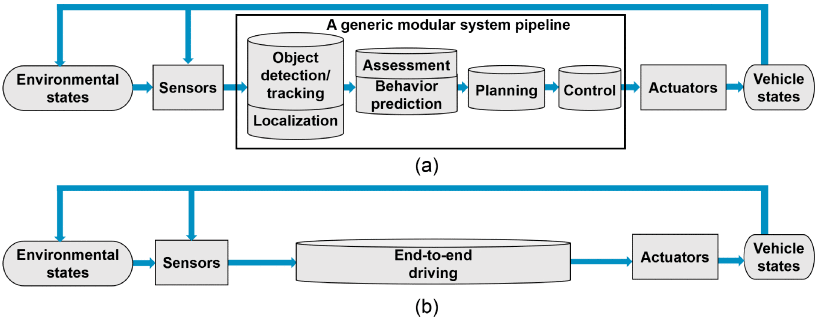
\includegraphics[width={0.9\textwidth}]{images/AD_architecture.png}
	\caption{Autonomous driving architecture: a) Modular system b) End-to-end system \cite{ad_pipeline}}
	\label{fig:ad_architercture}	
\end{figure}

%-----------
% Section 2: 
\subsection{Section 2}\label{sec:subsec_2.2}


% New sub-section:
% ----------------
\subsubsection{First sub-section under section 2}\label{ssec:subsubsec_2.2.1}



% New sub-section:
% ----------------
\subsubsection{Second sub-section under section2}\label{ssec:subsubsec_2.2.2}


% New sub-section:
% ----------------
\subsubsection{Third sub-section under section 2}\label{ssec:subsubsec_2.2.3}



%-----------
% Section 3: 
\subsection{Section 3}\label{sec:subsec_2.3}



%-----------
% Section 4: 
\subsection{Section 4}\label{sec:subsec_2.4}


% New sub-section:
% ----------------
\subsubsection{Uncertainty literature}\label{ssec:subsubsec_2.4.4}
By using equation \eqref{eqn:Gaussian processes} and equation \eqref{eqn:KL divergence} we can reference equations.

% Sample equation 1:
\def\A{
\begin{bmatrix}
   f(x_{1}) \\
   f(x_{2}) \\
   \vdots \\
   f(x_{m})
\end{bmatrix}
}

\def\B{
\begin{bmatrix}
    m(x_{1})\\
    m(x_{2}\\
    \vdots \\
    m(x_{m})
\end{bmatrix}
}

\def\C{
\begin{bmatrix}
    C(x_{1},x_{1}) \hdots C(x_{1},x_{m})\\
    C(x_{2},x_{1}) \hdots C(x_{2},x_{m})\\
    \vdots \\
    C(x_{m},x_{1}) \hdots C(x_{m},x_{m})
\end{bmatrix}
}
\begin{equation}\label{eqn:Gaussian processes}
    \A = \mathcal{N} \left(\B, \C\right)
\end{equation}

% Sample equation 2:
\begin{equation}\label{eqn:KL divergence}
    D_{KL}\{q_{\theta}(\theta) || p(\theta | X, Y)\} = \int q_{\theta}(\theta) \log \frac{q_{\theta}(\theta)}{p(\theta | X, Y)} d\theta
\end{equation}


%-----------
% Section 5: 
\subsection{Datasets}\label{sec:subsec_2.7}
By using table \ref{tbl:dataset}, we can reference tables.

% Sample table:
\begin{center}
\begin{tabular}{||c | c | c | c | c | c | c | c||} 
 \hline
 \thead{Dataset} & \thead{Scenes} & \thead{Sensors} & \thead{Anns.} & \thead{Map} & \thead{Rain/Night} & \thead{Classes} \\ [0.5ex]
 \hline\hline
 KITTI & 22 & Camera, LiDAR & 15,000 & No & No/No & 8\\ 
 \hline
 Waymo & 1150 & Camera, LiDAR & 200,000 & No & Yes/Yes & 4\\
 \hline
 nuScenes & 1000 & Camera, LiDAR, RADAR & 40,000 & Yes & Yes/Yes & 23\\ [1ex]
 \hline
\end{tabular}
\captionof{table}{Dataset comparison}
\label{tbl:dataset}
\end{center}

